\section{Sobolev Spaces of Functions with Gradients} \label{sec:3DGradSobSpaces}
In this section we deal with the details of the analysis of gradients of zero and tangential gradients with respect to the measures $\ddmes, \nu$, and $\dddmes$ --- our aim is to determine the behaviour of these objects and relate them to more familiar objects like weak derivatives.
Thematic throughout our analysis of gradients of zero and Sobolev functions will be the following procedure; we will first aim to understand gradients of zero on a single edge $I_{jk}$ that is parallel to (one of) the co-ordinate axes, and then employ rotation ideas to generalise our arguments to edges at any angle to the axes.
Next, we demonstrate that gradients of zero on $\graph$ can be built up from those on the individual edges --- this is unsurprising given that $\ddmes$ is just the sum of the individual singular measures supporting each edge.
Once we understand gradients of zero on edges, we can then understand the tangential gradients on the edges and on $\graph$ by following a similar line of reasoning --- working on the edges first and then looking at the implications for functions on the entire graph.
We will also have to consider (and analyse) the behaviour of gradients of zero and tangential gradients at the vertices, induced by $\nu$.
This finally allows us to understand Sobolev functions and their tangential gradients (and gradients of zero) on $\graph$ with respect to the measure $\dddmes$.
This approach will also guide us when we come to examine the Sobolev spaces of curls in section \tstk{ref!}.
As promised, we begin with an examination of gradients of zero.

\subsection{Gradients of Zero} \label{ssec:muGradZero}
In this section we will characterise gradients of zero with respect to the measures $\ddmes, \nu$, and $\dddmes$, in that order.
Throughout, we denote by $\ograd$ the $\ktgrad$ operator with $\kt=\bracs{0,0}$.
Given proposition \ref{prop:ZeroInvariantUnderQM-Wavenumber}, without loss of generality we can always take any approximating sequence $\phi_n$ for a gradient of zero $g$ to be such that $\ograd\phi_n\rightarrow g$, as opposed to $\ktgrad\phi_n\rightarrow g$.
\begin{prop}[Gradients of Zero on a Segment Parallel to the $x_2$-axis] \label{prop:3DGradZeroParallel}
	Suppose that the edge $I_{jk}$ is parallel to the $x_2$-axis.
	Then 
	\begin{align*}
		\gradZero{\ddom}{\lambda_{jk}} &= 
		\clbracs{ \bracs{g,0,0}^\top	\setVert g\in\ltwo{\ddom}{\lambda_{jk}} }.
	\end{align*}
\end{prop}
\begin{proof}
	This is a version of the argument in \cite[Section~3.1]{zhikov2000extension}, given proposition \ref{prop:GradZeroInvarientUnderQM} we can consider (without loss of generality) $\kt=\bracs{0,0}$ throughout.
	This argument is also one particular version of the argument in the proof of proposition \ref{prop:RotationOfEdgeGradients}, which we present in detail below.
\end{proof}

\begin{prop} \label{prop:3DGradZeroRotated}
	Let $I_{jk}$ be an edge of $\graph$.
	Then
	\begin{align*}
		\gradZero{\ddom}{\lambda_{jk}} 
		&= \clbracs{ g_{jk}\hat{n}_{jk} \setVert g_{jk}\in\ltwo{\ddom}{\lambda_{jk}} } \\
		&= \clbracs{ \begin{pmatrix} R_{jk}^{\top} & 0 \\ 0 & 1 \end{pmatrix} \bracs{g_{jk},0,0}^\top \setVert g_{jk}\in\ltwo{\ddom}{\lambda_{jk}} } \\
		&= \clbracs{ g_{jk}\in\ltwo{\ddom}{\ddmes}^2 \setVert g_{jk}\cdot e_{jk} = 0 }.
	\end{align*}
\end{prop}
Note that the three sets on the right hand side are all equal by definition of $n_{jk}, e_{jk}$, and $R_{jk}$.
As such, we will demonstrate the equality on the first line in the proof. 
\begin{proof}
	Clearly, if $g=\bracs{0,0,g_3}^\top\in\gradZero{\ddom}{\lambda_{jk}}$, then \eqref{eq:GradZeroSequenceDef} implies that $g_3=0$.
	
	Next, suppose that $g=g_{jk}\hat{e}_{jk}\in\gradZero{\ddom}{\lambda_{jk}}$, and take an approximating sequence $\phi_n$ for $g$.
	Given proposition \ref{prop:ZeroInvariantUnderQM-Wavenumber}, this implies that
	\begin{align*}
		\phi_n\lconv{\ltwo{\ddom}{\lambda_{jk}}}0, \quad
		\ograd\phi_n \lconv{\ltwo{\ddom}{\lambda_{jk}}^3} g\hat{e}_{jk}.
	\end{align*}
	Therefore, $\ograd\phi_n\cdot\hat{e}_{jk}\rightarrow g$, and thus
	\begin{align*}
		\int_0^{\abs{I_{jk}}} \abs{\diff{\phi_n}{y}\bracs{r_{jk}(y)} - g\bracs{r_{jk}(y)} }^2 \ \md y
		&= \integral{I_{jk}}{ \abs{\ograd\phi_n\cdot\hat{e}_{jk} - g}^2 }{\lambda_{jk}} \toInfty{n}, \\
		\implies \diff{\phi_n}{y}\bracs{r_{jk}(y)} &\lconv{\ltwo{\interval{I_{jk}}}{y}} g\bracs{r_{jk}(y)}.
	\end{align*}
	We also observe that $\phi_n\bracs{r_{jk}(y)}\rightarrow 0$ in $\ltwo{\interval{I_{jk}}}{y}$, and thus $g\bracs{r_{jk}(y)}$ is the derivative (in the classical $\gradSob{\interval{I_{jk}}}{y}$-sense) of the zero function, and thus $g=0$.
	
	Finally, suppose that $g\in\smooth{\ddom}$ and consider the smooth function $\phi(x) = \bracs{\bracs{x-v_j}\cdot n_{jk}}g(x)$.
	Then we have that $\ograd\phi_n = \bracs{\bracs{x-v_j}\cdot n_{jk}}\ograd g + g\hat{n}_{jk}$, and notice that $\bracs{x-v_j}\cdot n_{jk}	=0$ when $x\in I_{jk}$.
	It is now clear that $\phi=0$ and $\ograd\phi = g\hat{n}_{jk}$ on $I_{jk}$, so $g\hat{n}_{jk}\in\gradZero{\ddom}{\lambda_{jk}}$.
	By density of $\smooth{\ddom}$ in $\ltwo{\ddom}{\lambda_{jk}}$, we can conclude that $g\hat{n}_{jk}\in\gradZero{\ddom}{\lambda_{jk}}$ for every $g\in\ltwo{\ddom}{\lambda_{jk}}$.
\end{proof}
Taking $R_{jk}$ as the identity matrix to recover proposition \ref{prop:3DGradZeroParallel}.

We now focus on demonstrating that the set of gradients of zero on the entirety of $\graph$ is formed from gradients of zero on each edge.
That is, we look to prove the following characterisation of $\gradZero{\ddom}{\ddmes}$:
\begin{prop}[Characterisation of $\gradZero{\ddom}{\ddmes}$] \label{prop:3DGradZeroChar}
	For an embedded graph $\graph$ in $\ddom$, we have that
	\begin{align*}
		\gradZero{\ddom}{\ddmes} &= \clbracs{ g\in\ltwo{\ddom}{\ddmes}^3 \setVert g^{(jk)}\in\gradZero{\ddom}{\lambda_{jk}} \ \forall I_{jk}\in\edgeSet }.
	\end{align*}
\end{prop}
We will denote $B := \clbracs{ g\in\ltwo{\ddom}{\ddmes}^3 \setVert g^{(jk)}\in\gradZero{\ddom}{\lambda_{jk}} \ \forall I_{jk}\in\edgeSet }$ for the time being.
In order to prove proposition \ref{prop:3DGradZeroChar} we will need some supporting results, however the argument can be sketched out like so.
Showing that $\gradZero{\ddom}{\ddmes}\subset B$ is straightforward due to the definition of $\ddmes$ and that the norms we are interested in are related:
\begin{align*}
	\norm{\cdot}_{\ltwo{\ddom}{\lambda_{jk}}} &\leq \norm{\cdot}_{\ltwo{\ddom}{\ddmes}}, \\
	\norm{\cdot}_{\ltwo{\ddom}{\ddmes}}^2 &= \sum_{v_j\in\vertSet}\sum_{j\conLeft k}\norm{\cdot}_{\ltwo{\ddom}{\lambda_{jk}}}^2.
\end{align*}
The reverse inclusion is slightly more technical due to the fact that we have to form an approximating sequence (that converges on all of $\graph$) from a set of approximating sequences that each converge on one particular edge.
However we cannot simply extend an approximating sequence on an edge $I_{jk}$ by zero to the whole graph (as it is no longer guaranteed to be smooth), so have to smooth this sequence to zero over some small region around $I_{jk}$.
This ``smoothing" requires us to always have some non-zero distance between the edge $I_{jk}$ and all other edges of $\graph$, which is a non-trivial process if the support of the approximating sequence is close to one of the vertices $v_j$ or $v_k$.
Having overcome this obstacle, one can show that any $g_{jk}\in\gradZero{\ddom}{\lambda_{jk}}$ \emph{can} be extended by zero to obtain a function $g\in\gradZero{\ddom}{\ddmes}$, and then using linearity of the subspace $\gradZero{\ddom}{\ddmes}$, the proof will be complete.

Before continuing, we introduce two families of smooth functions that we shall make use of during the proof of proposition \ref{prop:3DGradZeroChar}.
Let $\eta\in\smooth{\ddom}$ have the properties
\begin{align*}
	0 \leq \eta(x) \leq 1, \quad
	\eta(x) = 0 \text{ when } \abs{x} \leq 1, \quad
	\eta(x) = 1 \text{ when } \abs{x} \geq 2.
\end{align*}
Then define
\begin{align} \label{eq:SmoothEtaDef}
	\eta_j(x) = \eta\bracs{x-v_j}, \quad
	\eta_j^n(x) = \eta_j\bracs{nx},
\end{align}
which are both smooth functions by composition.
The functions $\eta_j^n$ will enable us to extend functions defined on one edge $I_{jk}$ to the whole of $\graph$ without worrying about proximity to the vertex $v_j$.
Notice that $\eta_j^n\rightarrow 1 \toInfty{n}$ in $\ltwo{\ddom}{\ddmes}$ since
\begin{align*}
	\integral{\ddom}{ \abs{\eta_j^n - 1}^2 }{\ddmes} &\leq
	\integral{ B_{2/n}\bracs{v_j} }{}{\ddmes}
	= \ddmes\bracs{ B_{2/n}\bracs{v_j} } \leq \frac{4\abs{\edgeSet}}{n}.
\end{align*}
Additionally, we have that $\eta_j^n$ also converges in $\ltwo{\ddom}{\dddmes}$ to the function
\begin{align*}
	\tilde{\charFunc{j}} = \begin{cases} 1 & x\neq v_j, \\ 0 & x=v_j, \end{cases}
\end{align*}
since
\begin{align*}
	\norm{\eta_j^n - \tilde{\charFunc{j}}}_{\ltwo{\ddom}{\ddmes}}^2
	&= \norm{\eta_j^n - 1}_{\ltwo{\ddom}{\ddmes}}^2
	+ \integral{\ddom\setminus\clbracs{v_j}}{ \abs{\eta_j^n - 1}^2 }{\nu} \\
	&= \norm{\eta_j^n - 1}_{\ltwo{\ddom}{\ddmes}}^2 \rightarrow 0.
\end{align*}
Unsurprisingly we also need a family of smooth functions to help us ``smooth off" any approximating sequences.
Let $I_{jk}\in\edgeSet$, $\eps>0$, and set
\begin{align} \label{eq:ShortenedEdgeDef}
	I_{jk}^\eps := \clbracs{ x\in I_{jk} \setVert \mathrm{dist}\bracs{x,\partial I_{jk}}\geq\recip{\eps} }.
\end{align}
Let $\chi_{jk}^\eps\in\smooth{\ddom}$ be such that
\begin{align} \label{eq:SmoothChiDef}
	0 \leq \chi_{jk}^n \leq 1, \quad
	\chi_{jk}^\eps(x) = 1 \text{ when } \mathrm{dist}\bracs{x, I_{jk}^\eps}\leq \recip{3\eps}, \quad
	\chi_{jk}^\eps(x) = 0 \text{ when } \mathrm{dist}\bracs{x, I_{jk}^\eps}\geq \frac{2}{3\eps}.
\end{align}
As $\graph$ is finite, we can assume without loss of generality that the only edge of $\graph$ that $\supp\bracs{\chi_{jk}^\eps}$ intersect is $I_{jk}$ (otherwise, we just rescale the argument).
We can also assemble $\chi_{jk}^\eps$ such that $\abs{ \ograd\chi_{jk}^{\eps} } \leq c\eps$ for some $c\geq 0$ independent of $\eps$.
We can check the convergence of $\chi_{jk}^\eps \toInfty{\eps}$ in $\ltwo{\ddom}{\ddmes}$ to the characteristic function of the edge $I_{jk}$, denoted by $\charFunc{jk}$;
\begin{align*}
	\integral{\ddom}{ \abs{\chi_{jk}^\eps - \charFunc{jk}}^2 }{\ddmes}
	&= \integral{I_{jk}}{ \abs{\chi_{jk}^\eps - \charFunc{jk}}^2 }{\lambda_{jk}}
	\leq \integral{I_{jk}\cap\clbracs{\chi_{jk}^\eps\leq 1}}{}{\lambda_{jk}}
	= \frac{2}{3\eps} \rightarrow 0 \toInfty{\eps}.
\end{align*}
We also have that $\chi_{jk}^\eps$ converges to the characteristic function $\charFunc{jk}^\circ$ of the interior of $I_{jk}$ in $\ltwo{\ddom}{\dddmes}$, since
\begin{align*}
	\integral{\ddom}{ \abs{\chi_{jk}^\eps - \charFunc{jk}^\circ}^2 }{\dddmes}
	&= \integral{\ddom}{ \abs{\chi_{jk}^\eps - \charFunc{jk}^\circ}^2 }{\ddmes}
	= \integral{\ddom}{ \abs{\chi_{jk}^\eps - \charFunc{jk}}^2 }{\ddmes}.
\end{align*}

We can now prove proposition \ref{prop:3DGradZeroChar} --- the inclusion $\gradZero{\ddom}{\ddmes}\subset B$ follows immediately.
\begin{lemma} \label{lem:3DGradZeroSubsetB}
	\begin{align*}
		\gradZero{\ddom}{\ddmes} \subset B.
	\end{align*}
\end{lemma}
\begin{proof}
	This is a direct consequence of $\lambda_{jk}$ being a restriction of $\ddmes$ to a given edge.
	Indeed, let $g\in\gradZero{\ddom}{\ddmes}$ and let $\phi_n$ be an approximating sequence for $g$.
	Then clearly
	\begin{align*}
		\norm{\phi_n}_{\ltwo{\ddom}{\lambda_{jk}}} &\leq \norm{\phi_n}_{\ltwo{\ddom}{\ddmes}} \rightarrow 0, \\
		\norm{\ograd\phi_n - g^{(jk)}}_{\ltwo{\ddom}{\lambda_{jk}}} &\leq \norm{\ograd\phi_n - g}_{\ltwo{\ddom}{\ddmes}} \rightarrow 0,
	\end{align*}
	thus $g\in\ltwo{\ddom}{\lambda_{jk}}$ for every $I_{jk}$, so $g\in B$.
\end{proof}
Turning our attention to the reverse inclusion, we first demonstrate that so long as a gradient of zero on an edge $I_{jk}$ has support contained within the interior of the $I_{jk}$, we can extend it to a gradient of zero on the whole graph.
\begin{lemma}[Extension lemma for Gradients of Zero] \label{lem:3DExtensionLemmaGrads}
	Let $n\in\naturals$ and $I_{jk}^n$ be as in \eqref{eq:ShortenedEdgeDef}.
	Suppose that $g_{jk}\in\gradZero{\ddom}{\lambda_{jk}}$ with $\supp\bracs{g_{jk}}\subset I_{jk}^n$.
	Define the functions $g\in\ltwo{\ddom}{\ddmes}$ and $\tilde{g}\in\ltwo{\ddom}{\dddmes}$ by
	\begin{align*}
		g =	\begin{cases} g_{jk} & \mathrm{on} \ I_{jk}, \\ 0 & \mathrm{otherwise}, \end{cases} 
		&\quad
		\tilde{g} =	\begin{cases} g_{jk} & \mathrm{on} \ I_{jk}\setminus\clbracs{v_j,v_k}, \\ 0 & \mathrm{otherwise}. \end{cases}
	\end{align*}
	Then $g\in\gradZero{\ddom}{\ddmes}$ and $\tilde{g}\in\gradZero{\ddom}{\dddmes}$.
\end{lemma}
\begin{proof}
	Let $\phi_n$ be an approximating sequence for $g_{jk}$, and consider the sequence (of smooth functions) $\psi_l = \chi_{jk}^n\phi_l$.
	We have that
	\begin{align*}
		\norm{\psi_l}_{\ltwo{\ddom}{\ddmes}} 
		&= \norm{\chi_{jk}^n\phi_l}_{\ltwo{\ddom}{\lambda_{jk}}}
		\leq \norm{\phi_l}_{\ltwo{\ddom}{\lambda_{jk}}} \rightarrow 0 \toInfty{l}.
	\end{align*}
	Furthermore,
	\begin{align*}
		\norm{\ograd\psi_l - g}_{\ltwo{\ddom}{\ddmes}^2}^2
		&= \norm{\chi_{jk}^n\ograd\phi_l + \phi_l\ograd\chi_{jk}^n - g_{jk}}_{\ltwo{\ddom}{\lambda_{jk}}^2}^2 \\
		&\leq 2\norm{\phi_l\ograd\chi_{jk}^n}_{\ltwo{\ddom}{\lambda_{jk}}^2}^2 + 2\norm{\chi_{jk}^n\ograd\phi_l - g_{jk}}_{\ltwo{\ddom}{\lambda_{jk}}^2}^2 \\
		&\leq 2\sup_{I_{jk}}\abs{\ograd\chi_{jk}^n}^2 \norm{\phi_l}_{\ltwo{\ddom}{\lambda_{jk}}^2}^2
		+ 2\norm{\ograd\phi_l - g_{jk}}_{\ltwo{\ddom}{\lambda_{jk}}^2}^2 \\
		&\rightarrow 0 \toInfty{l}.
	\end{align*}
	Therefore, $\psi_l$ is an approximating sequence for $g$, and thus $g\in\gradZero{\ddom}{\ddmes}$, as required.
	
	Next, notice that $\psi_l\bracs{v_j} = \psi_l\bracs{v_k} = 0$, and $\ograd\psi_l\bracs{v_j} = \ograd\psi_l\bracs{v_k} = 0$ for every $l\in\naturals$.
	Therefore,
	\begin{align*}
		\norm{\psi_l}_{\ltwo{\ddom}{\nu}} = 0 = \norm{\ograd\psi_l}_{\ltwo{\ddom}{\nu}^2},
	\end{align*}
	for every $l\in\naturals$, and so
	\begin{align*}
		\norm{\psi_l}_{\ltwo{\ddom}{\dddmes}} &= \norm{\psi_l}_{\ltwo{\ddom}{\ddmes}} \rightarrow 0, \\
		\norm{\ograd\psi_l - \tilde{g}}_{\ltwo{\ddom}{\dddmes}^2} &= \norm{\ograd\psi_l - g}_{\ltwo{\ddom}{\ddmes}^2}^2 \rightarrow 0,
	\end{align*}
	and thus $\tilde{g}\in\gradZero{\ddom}{\dddmes}$.
\end{proof}
The hypothesis that $\supp\bracs{g_{jk}}\subset I_{jk}^n$ is essential for the inequality 
\begin{align*}
	\norm{\ograd\phi_l - g_{jk}}_{\ltwo{\ddom}{\lambda_{jk}}^2} \leq \norm{\ograd\phi_l - g_{jk}}_{\ltwo{\ddom}{\lambda_{jk}}^2}
\end{align*} 
to hold, and so that we can use the function $\chi_{jk}^n$ to ensure that our approximating sequence $\psi_l$ is ``restricted" to the edge $I_{jk}$ only, on which we know that $\phi_l$ has the properties we need.

We can now use the fact that the space of gradients of zero is closed to complete the proof of proposition \ref{prop:3DGradZeroChar}.
\begin{prop} \label{prop:3DBSubsetGradZero}
	We have that
	\begin{align*}
		\gradZero{\ddom}{\ddmes} \supset B.
	\end{align*}
	Furthermore, for any $g\in B$, let $\tilde{g}\in\ltwo{\ddom}{\dddmes}$ be defined by
	\begin{align*}
		\tilde{g}(x) &= \begin{cases} 0 & x\in\vertSet, \\ g & \mathrm{otherwise}. \end{cases}
	\end{align*}
	Then $\tilde{g}\in\gradZero{\ddom}{\dddmes}$.
\end{prop}
\begin{proof}
	Let $g\in B$, and define a family of functions $g_n$ by
	\begin{align*}
		g_n &= \sum_{v_j\in\vertSet}\sum_{j\conLeft k}\eta_j^n \eta_k^n g^{(jk)}.
	\end{align*}
	The graph $\graph$ is finite, so the sum converges.
	For each $j,k$ in the sum, the function $\eta_j^n \eta_k^n g^{(jk)}$ is an element of $\ltwo{\ddom}{\lambda_{jk}}$ with support in $I_{jk}^n$, so satisfies the hypothesis of the Extension lemma \ref{lem:3DExtensionLemmaGrads}.
	Therefore, $\eta_j^n \eta_k^n g^{(jk)}\in\gradZero{\ddom}{\ddmes}$ and since $\gradZero{\ddom}{\ddmes}$ is a linear subspace, $g_n\in\gradZero{\ddom}{\ddmes}$ for every $n\in\naturals$.
	Furthermore, we can see that $g_n\rightarrow g \toInfty{n}$ in $\ltwo{\ddom}{\ddmes}$ by the algebra of limits.
	Since $\gradZero{\ddom}{\ddmes}$ is closed, we conclude that $g\in\gradZero{\ddom}{\ddmes}$ too.
	
	Similarly, we can conclude by the Extension lemma \ref{lem:3DExtensionLemmaGrads} that the functions
	\begin{align*}
		\tilde{g}_n &= \begin{cases} 0 & x\in\vertSet, \\ g_n & \mathrm{otherwise}, \end{cases}
	\end{align*}
	form elements of $\gradZero{\ddom}{\dddmes}$ for each $n\in\naturals$.
	In addition, $\tilde{g}_n$ converges to $\tilde{g}$, and by closure, we have $\tilde{g}\in\gradZero{\ddom}{\dddmes}$.
\end{proof}
Proposition \ref{prop:3DBSubsetGradZero} and lemma \ref{lem:3DGradZeroSubsetB} then constitute the proof of proposition \ref{prop:3DGradZeroChar}.
The fact that we can also extend elements of $\gradZero{\ddom}{\ddmes}$, and hence $\gradZero{\ddom}{\lambda_{jk}}$, to elements of $\gradZero{\ddom}{\dddmes}$ will also contribute to our characterisation of the set $\gradZero{\ddom}{\dddmes}$.

Having dealt with the behaviour of gradients of zero on the edges of the graph $\graph$, we turn our attention to their behaviour at the vertices, induced by the measure $\nu$.
This analysis is far more straightforward than for $\ddmes$, in no small part due to the fact that the vertices of $\graph$ are isolated from each other, and so there are no problems centred around one vertex's proximity to another.
Let us begin by defining some useful functions and constants.
Set 
\begin{align} \label{eq:HalfMinDistBetweenVertsDef}
	d := \recip{2}\min\clbracs{\abs{I_{jk}} \setVert I_{jk}\in\edgeSet},
\end{align}
which exists and is strictly greater than 0 since $\graph$ is finite.
For $c\in\complex$, let $\varphi_c:\reals^2\rightarrow\complex$ be a smooth function such that
\begin{align} \label{eq:NuSmoothVertexFunctionDef}
	\varphi_c(0) = 0, \quad
	\grad\varphi_c(0) = c, \quad
	\supp\bracs{\varphi_c}\subset B_d(0),
\end{align}
where $B_d(0)$ is the ball of radius $d$ centred at the origin.
Finally, set $N = \abs{\vertSet}$ and for each $v_j\in\vertSet$ define
\begin{align*}
	g_1^j(x) = \begin{cases} \bracs{1,0,0}^\top, & x=v_j, \\ 0 & x\neq v_j, \end{cases}
	\quad
	g_2^j(x) = \begin{cases} \bracs{0,1,0}^\top, & x=v_j, \\ 0 & x\neq v_j, \end{cases}
	\quad
	g_3^j(x) = \begin{cases} \bracs{0,0,1}^\top, & x=v_j, \\ 0 & x\neq v_j. \end{cases}
\end{align*}
We will now demonstrate that $\ltwo{\ddom}{\nu}^3$ is isomorphic to $\complex^{3N}$. 
\begin{lemma} \label{lem:L2nuIsomCN}
	The space $\ltwo{\ddom}{\nu}^3$ is isomorphic to $\complex^{3N}$.
	Furthermore, the collection 
	\begin{align*}
		B_{\nu} = \clbracs{g_1^j, g_2^j, g_3^j \setVert v_j\in\vertSet}
	\end{align*} forms a basis of $\ltwo{\ddom}{\nu}^3$.
\end{lemma}
\begin{proof}
	It is sufficient to notice that any $f\in\ltwo{\ddom}{\nu}^3$ is entirely determined by the values it takes at the vertices $v_j$.
	As such, we can define the map
	\begin{align*}
		\iota:\ltwo{\ddom}{\nu} \rightarrow \complex^{3N}, \quad
		\iota(f) = \bracs{\frac{f\bracs{v_1}}{\sqrt{\alpha_1}}, \frac{f\bracs{v_2}}{\sqrt{\alpha_2}}, \hdots, \frac{f\bracs{v_N}}{\sqrt{\alpha_N}}}^\top,
	\end{align*}
	where we have vertically concatenated the collection of three-vectors $f\bracs{v_j}, v_j\in\vertSet$ 	(and use the principle square root if $\alpha_j$ has non-zero imaginary part).
	Clearly $\iota$ is a bijection, and additionally for $f,g\in\ltwo{\ddom}{\nu}^3$ we have that
	\begin{align*}
		\ip{f}{g}_{\ltwo{\ddom}{\nu}^3} &= \integral{\ddom}{f\cdot\overline{g}}{\nu}
		= \sum_{v_j\in\vertSet}\alpha_j f\bracs{v_j}\overline{g\bracs{v_j}}
		= \iota(f)\cdot\overline{\iota(g)}
		= \ip{\iota(f)}{\iota(g)}_{\complex^{3N}},
	\end{align*}
	so $\iota$ is an isometry.
	Furthermore, the image of $B_{\nu}$ under $\iota$ is the canonical basis of $\complex^{3N}$, and thus the collection $B_{\nu}$ forms a basis of $\ltwo{\ddom}{\nu}^3$.
\end{proof}
Of course, if any of the $\alpha_j=0$, then we have that $\ltwo{\ddom}{\nu}^2$ is isomorphic to $\complex^{2(N-M)}$, where there are $M$ such $\alpha_j=0$ --- the obvious adjustment can be made to the map $\iota$.

The reason for observing that the collection $B_{\nu}$ is a basis of $\ltwo{\ddom}{\nu}^3$ is so that characterising the space $\gradZero{\ddom}{\nu}$ is now an easy task.
\begin{prop} \label{prop:NuGradZeroChar}
	We have that 
	\begin{align*}
		\gradZero{\ddom}{\nu} &= \mathrm{span}\clbracs{g_1^j, g_2^j \setVert j\in\vertSet }
		= \clbracs{ g\in\ltwo{\ddom}{\nu}^3 \setVert g_3 = 0}.
	\end{align*}
\end{prop}
\begin{proof}
	Notice that for any $g\in\gradZero{\ddom}{\nu}$, any approximating sequence $\phi_n$ is such that
	\begin{align*}
		\phi_n \rightarrow 0, \quad \partial_1\phi_n \rightarrow g_1, 
		\quad \partial_2\phi_n\rightarrow g_2, \quad \rmi\wavenumber\phi_n \rightarrow g_3,
	\end{align*}
	and therefore $g_3 = 0$ since $\rmi\wavenumber\phi_n$ converges to $g_3$ and the zero function.
	
	Now take $c=\bracs{1,0,0}^\top$ and $v_j\in\vertSet$, and let $\phi(x) = \varphi_c\bracs{x-v_j}$ for $\varphi_c$ as in \eqref{eq:NuSmoothVertexFunctionDef}.
	The function $\phi$ is smooth, has support contained in $B_d\bracs{v_j}$, and is such that $\ograd\phi(x) = \ograd\varphi_c\bracs{x-v_j}$.
	Clearly
	\begin{align*}
		\integral{\ddom}{\abs{\phi}^2}{\nu} = 0, \quad
		\integral{\ddom}{\abs{\ograd\phi - g_1^j}^2}{\nu} = 0,
	\end{align*}
	hence $g_1^j\in\gradZero{\ddom}{\nu}$.
	By a similar construction, we can show that $g_2^j\in\gradZero{\ddom}{\nu}$ too, and since $\gradZero{\ddom}{\nu}$ is a closed linear subspace of $\ltwo{\ddom}{\nu}^3$, we have the desired result.
\end{proof}

Given that the measure $\dddmes = \ddmes + \nu$, propositions \ref{prop:3DGradZeroChar} and \ref{prop:NuGradZeroChar} allow us to understand $\gradZero{\ddom}{\dddmes}$.
Intuitively, $\gradZero{\ddom}{\dddmes}$ is made up of linear combinations of gradients of zero with respect to $\ddmes$ and $\nu$, although we will qualify this statement since the functions (or rather, equivalence classes of functions) that live in $\gradZero{\ddom}{\ddmes}$ and $\gradZero{\ddom}{\nu}$ are defined on different parts of $\graph$.
\begin{theorem}[``Characterisation" of $\gradZero{\ddom}{\dddmes}$] \label{thm:3DdddmesCharGradZero}
	Let $\tilde{g}\in\ltwo{\ddom}{\dddmes}^3$ and define
	\begin{align*}
		g_\mu(x) = \begin{cases} \tilde{g}(x) & x\neq v_j, \ \forall v_j\in\vertSet, \\ 0 & x=v_j, \ v_j\in\vertSet, \end{cases}
		\qquad
		g_\nu(x) = \begin{cases} 0 & x\neq v_j, \ \forall v_j\in\vertSet, \\ \tilde{g}\bracs{v_j} & x=v_j, \ v_j\in\vertSet, \end{cases}
	\end{align*}
	so $\tilde{g} = g_\mu + g_\nu$ (in $\ltwo{\ddom}{\dddmes}^3$).
	Then
	\begin{align*}
		\tilde{g}\in\gradZero{\ddom}{\dddmes} \quad\Leftrightarrow\quad
		g_\mu\in\gradZero{\ddom}{\ddmes} \text{ and } g_\nu\in\gradZero{\ddom}{\nu}.
	\end{align*}
\end{theorem}
\begin{proof}
	$\bracs{\Rightarrow}$ For the right-directed implication, it is sufficient to notice that
	\begin{align*}
		\norm{\cdot}_{\ltwo{\ddom}{\dddmes}^3}^2 &= \norm{\cdot}_{\ltwo{\ddom}{\ddmes}^3}^2 + \norm{\cdot}_{\ltwo{\ddom}{\nu}^3}^2,
	\end{align*}
	so any approximating sequence for $\tilde{g}$ also converges to $g_\mu$ in $\ltwo{\ddom}{\ddmes}^3$ and $g_\nu$ in $\ltwo{\ddom}{\nu}^3$.
	
	$\bracs{\Leftarrow}$ For the left-directed implication, it will be sufficient for us to show the result holds when $g_\mu=0$ and then for when $g_\nu=0$, since we can use linearity of $\gradZero{\ddom}{\dddmes}$ to then complete the proof.
	With this in mind, notice that the Extension lemma \ref{lem:3DExtensionLemmaGrads} and proposition \ref{prop:3DBSubsetGradZero} deal with the case $g_\nu=0$, demonstrating that $\tilde{g}\in\gradZero{\ddom}{\dddmes}$.
	For the case when $g_\mu=0$, we can again take without loss of generality $g_\nu$ to be non-zero at exactly one vertex $v_j\in\vertSet$ (as again, we can then use linearity of $\gradZero{\ddom}{\dddmes}$).
	Let this be the case, so $g_\mu=0$ and $g_\nu=0$ except at the vertex $v=\bracs{v_1,v_2}^\top\in\vertSet$, where $g_\nu(v) =: g = \bracs{g_1,g_2,0}^\top$.
	Consider smooth functions $\phi_n$ for each $n\in\naturals$ where
	\begin{align*}
		\phi_n(x) &= \bracs{x_1-v_1}g_1 + \bracs{x_2-v_2}g_2, &\text{when } \abs{x-v}\leq\recip{n}, \\
		\phi_n(x) &= 0, &\text{when } \abs{x-v}\geq\frac{2}{n}.
	\end{align*}
	Note that $\phi_n(v)=0$ and $\grad\phi_n(v)=g$ for every $n\in\naturals$.
	Since $\abs{\phi_n(x)}\leq\recip{n}\abs{g_\nu(v)}$ when $\abs{x-v}=\recip{n}$, we can also chose $\phi_n$ so that there exists a constant $c$ independent of $n$ such that $\abs{\grad\phi_n(x)}\leq c\abs{g_\nu(v)}$ whenever $\recip{n}\leq\abs{x-v}\leq\frac{2}{n}$.
	Then
	\begin{align*}
		\integral{\ddom}{ \abs{\phi_n}^2 }{\dddmes}
		&= \integral{B_{2/n}(v)}{ \abs{\phi_n}^2 }{\ddmes} + \alpha_v\abs{\phi_n(v)}^2
		\leq \integral{B_{2/n}(v)}{ \recip{n^2}\abs{g}^2 }{\ddmes} \\
		&= \frac{2\abs{g}^2 \mathrm{deg}(v)}{n^3} \rightarrow 0, \\
		\integral{\ddom}{ \abs{\ograd\phi_n - \tilde{g}}^2 }{\dddmes}
		&= \integral{B_{2/n}(v)}{ \abs{\ograd\phi_n}^2 }{\ddmes} + \alpha_v\abs{\ograd\phi_n(v) - g}^2
		\leq c\abs{g}^2\integral{B_{2/n}(v)}{}{\ddmes} \\
		&= \frac{2c\abs{g}^2\mathrm{deg}(v)}{n} \rightarrow 0,
	\end{align*}
	where $\mathrm{deg}(v)$ denotes the degree of the vertex $v$.
	The sequence $\phi_n$ thus serves as an approximating sequence for $g_\nu$, so $g_\nu\in\gradZero{\ddom}{\dddmes}$, and since $\gradZero{\ddom}{\dddmes}$ is a linear subspace, the proof is complete.
\end{proof}

\subsection{Tangential Gradients} \label{ssec:3DTangGradients}
Thanks to theorem \ref{thm:3DdddmesCharGradZero}, we have an explicit description of gradients of zero with respect to $\dddmes$.
This will allow us to determine the form of the tangential gradients that functions $u\in\ktgradSob{\ddom}{\dddmes}$ due to the requirement that they be orthogonal to $\gradZero{\ddom}{\dddmes}$.
We will begin by studying tangential gradients with respect to $\ddmes$ and $\nu$, since theorem \ref{thm:3DdddmesCharGradZero} will then allow us to use this information in deducing the form of tangential gradients with respect to $\dddmes$.
\begin{prop} \label{prop:3DTangGradParallel}
	\sloppy Suppose that the edge $I_{jk}$ is parallel to the $x_2$-axis, and that $u\in\ktgradSob{\ddom}{\lambda_{jk}}$.
	Let $\widetilde{u} = u\circ r_{jk}$.
	Then $\widetilde{u}\in\gradSob{\interval{I_{jk}}}{y}$ and
	\begin{align*}
		\ktgrad_{\lambda_{jk}}u = 
		\begin{pmatrix}
			0 \\ u' + \rmi\qm_2 u \\ \rmi\wavenumber u
		\end{pmatrix},
	\end{align*}
	where $u' := \widetilde{u}'\circ r_{jk}^{-1}$.
\end{prop}
The proof is a special case of the argument presented for the result which follows.
Given the association between $\ltwo{\ddom}{\lambda_{jk}}$ and $\ltwo{\interval{I_{jk}}}{y}$, we have elected to use prime notation $u'$ to indicate that $u$ possesses some (analogue of) a classical derivative (almost everywhere).
This is of course due to $\widetilde{u}\in\gradSob{\interval{I_{jk}}}{y}$ being (almost everywhere) absolutely continuous. \tstk{Evan's PDE book is a good reference for this}
The function $\widetilde{u}$ also possesses a trace into $y=0$ and $y=\abs{I_{jk}}$, and so $u$ also has well-defined traces onto the vertices $v_j$ and $v_k$ \emph{from the edge $I_{jk}$}.
Importantly though, $u'$ is only a ``derivative" on the edge $I_{jk}$ --- there is no a priori requirement that these derivatives (or even $u$ itself) behave at shared vertices.
For example, if a vertex $v_j$ is shared between two edges $I_{jk}$ and $I_{jl}$, there is no guarantee that that the traces $u_{jk}\bracs{v_j}$ and $u_{jl}\bracs{v_l}$ coincide. 
We shall address this matter when we come to look at tangential gradients with respect to $\ddmes$.

\begin{cory} \label{cory:3DTangGradRotated}
	Let $I_{jk}\in\edgeSet$ and suppose that $u\in\ktgradSob{\ddom}{\lambda_{jk}}$.
	Set $\widetilde{u} = u\circ r_{jk}$.
	Then $u\in\gradSob{\interval{I_{jk}}}{y}$ and 
	\begin{align*}
		\ktgrad_{\lambda_{jk}}u = \bracs{u'+\rmi\qm_{jk}u}\hat{e}_{jk} + \rmi\wavenumber u\hat{x}_3,
	\end{align*}
	where $\qm_{jk}:=\qm\cdot e_{jk} = \bracs{R_{jk}\qm}_2$, and $u' = \widetilde{u}'\circ r_{jk}^{-1}$.
\end{cory}
\begin{proof}
	Since $\ktgrad_{\lambda_{jk}}u$ is orthogonal to $\gradZero{\ddom}{\lambda_{jk}}$ and given proposition \ref{prop:3DGradZeroRotated}, we have that for any $g\in\ltwo{\ddom}{\lambda_{jk}}$,
	\begin{align*}
		0 &= \integral{\ddom}{ \ktgrad_{\lambda_{jk}}u \cdot \overline{g}\hat{n}_{jk} }{\lambda_{jk}}
		= \integral{\ddom}{ \overline{g}\bracs{\ktgrad_{\lambda_{jk}}u\cdot\hat{n}_{jk}} }{\lambda_{jk}},
	\end{align*}
	and so $\ktgrad_{\lambda_{jk}}u\cdot\hat{n}_{jk}=0$.
	As such, we can write
	\begin{align*}
		\ktgrad_{\lambda_{jk}}u = v_{jk}\hat{e}_{jk} + v_3\hat{x}_3,
	\end{align*}
	for some $v_{jk},v_3\in\ltwo{\ddom}{\lambda_{jk}}$.
	Now take an approximating sequence for $\phi_n$ for $u$, so the following convergences (in $\ltwo{\ddom}{\lambda_{jk}}$) hold
	\begin{align*}
		\phi_n \rightarrow u, \quad 
		\begin{pmatrix}
			\bracs{ \partial_1 + \rmi\qm_1 }\phi_n \\
			\bracs{ \partial_2 + \rmi\qm_2 }\phi_n \\
			\rmi\wavenumber\phi_n
		\end{pmatrix}
		\rightarrow v_{jk}\hat{e}_{jk} + v_3\hat{x}_3.
	\end{align*}
	Clearly we must have that $v_3 = \rmi\wavenumber u$.
	Additionally, we have that
	\begin{align*}
		\begin{pmatrix}
			\bracs{ \partial_1 + \rmi\qm_1 }\phi_n \\
			\bracs{ \partial_2 + \rmi\qm_2 }\phi_n
		\end{pmatrix}
		\rightarrow v_{jk}e_{jk},
		\quad \implies
		\begin{pmatrix}
			\partial_1\phi_n \\
			\partial_2\phi_n
		\end{pmatrix}
		\cdot e_{jk}
		\rightarrow v_{jk} - \rmi\bracs{\qm\cdot e_{jk}}u = v_{jk} - \rmi\qm_{jk}u
	\end{align*}
	Write $\widetilde{\phi}_n = \phi_n\circ r_{jk}$ and $\widetilde{v}_{jk}=v_{jk}\circ r_{jk}$, then the above implies that
	\begin{align*}
		\int_0^{\abs{I_{jk}}} \abs{ \widetilde{\phi}_n'(y) - \widetilde{v}_{jk}(y) + \rmi\qm_{jk}  }^2
		&= \integral{\ddom}{ \abs{ \grad\phi_n\cdot e_{jk} - v_{jk} + \rmi\qm_{jk}u }^2 }{\lambda_{jk}} \\
		&\rightarrow 0 \toInfty{n}.
	\end{align*}
	We can also deduce that $\widetilde{\phi}_n\rightarrow \widetilde{u}$ in $\ltwo{\interval{I_{jk}}}{y}$ too, which implies that $\widetilde{u}\in\gradSob{\interval{I_{jk}}}{y}$ with $\widetilde{u}' = \widetilde{v}_{jk} - \rmi\qm_{jk}\widetilde{u}$.
	Rearranging for $\widetilde{v}_{jk}$ and undoing the change of variables $r_{jk}$ then provides the result.
\end{proof}

Corollary \ref{cory:3DTangGradRotated} provides us with an explicit expression for the tangential gradient of a function on one edge of $\graph$.
Given that proposition \ref{prop:3DGradZeroChar} informs us that the set of gradients of zero on $\graph$ can be formed from combining gradients of zero on each edge, we can now obtain an expression for $\ktgrad_{\ddmes}u$ on any edge $I_{jk}$.
However, this is not all that can be deduced about functions $u\in\ktgradSob{\ddom}{\ddmes}$ --- we can also address the issue of the value that $u$ should take at the vertices of $\graph$.
Given that $u$ possesses a trace from each edge into the vertices, we should expect a matching condition to relate these traces at vertices common to multiple edges.
Indeed, we will see that $u$ must be continuous at the vertices --- that is, the trace of $u$ from each edge into a common vertex are identical.
\begin{theorem} \label{thm:3DTangGradGraph}
	We have that
	\begin{align*}
		u\in\ktgradSob{\ddom}{\ddmes} \quad\Rightarrow\quad
		\begin{cases}
			\mathrm{(i)} \ u\in\ktgradSob{\ddom}{\lambda_{jk}}, & \forall I_{jk}\in\edgeSet, \\
			\mathrm{(ii)} \ \ktgrad_{\ddmes}u = \ktgrad_{\lambda_{jk}}u, & \text{on every } I_{jk}, \\
			\mathrm{(iii)} \ u \text{ is continuous at } v_j, & \forall v_j\in\vertSet.
		\end{cases}
	\end{align*}
\end{theorem}
\tstk{Zhikov converse mention, claims converse holds but only gives elasticity case proof, and uses a proposition which seems like it's just wrong}
Our approach is as follows; first we show that (i) and (ii) hold by appealing to an approximating sequence and using proposition \ref{prop:3DGradZeroChar}.
For (iii), we also demonstrate that any approximating sequence for $u$ is also Cauchy in the uniform norm on each edge $I_{jk}$, and so must converge by completeness of the uniform norm, and the limit must be $u^{(jk)}$.
This will be enough to deduce that $\phi_n$ converges uniformly on the ``junction region" surrounding each vertex $v_j$, and since $\phi_n$ is chosen to be continuous over all of $\ddom$, we will obtain continuity of $u$ at the vertices.
\begin{proof}
	Suppose $u\in\ktgradSob{\ddom}{\ddmes}$ and let $\phi_n$ be an approximating sequence for $u$.
	Since $\norm{\cdot}_{\ltwo{\ddom}{\lambda_{jk}}} \leq \norm{\cdot}_{\ltwo{\ddom}{\ddmes}}$, we have that 
	\begin{align} \label{eq:3DTangGradProofApproxSequence}
		\phi_n\lconv{\ltwo{\ddom}{\lambda_{jk}}} u, 
		\quad
		\ktgrad\phi_n\lconv{\ltwo{\ddom}{\lambda_{jk}}^3}\ktgrad_{\ddmes}u,
	\end{align}
	and so $u\in\ktgradSob{\ddom}{\lambda_{jk}}$ by definition.
	To show that $\ktgrad_{\ddmes}u = \ktgrad_{\lambda_{jk}}u$ on $I_{jk}$, we must show that $\ktgrad_{\ddmes}u$ is orthogonal to $\gradZero{\ddom}{\lambda_{jk}}$ (and then by uniqueness of tangential gradients the desired equality follows).
	So take any $g\in\gradZero{\ddom}{\lambda_{jk}}$; we have that the function
	\begin{align*}
		\widetilde{g} = \begin{cases} g & x\in I_{jk}, \\ 0 & x\not\in I_{jk} \end{cases}
	\end{align*}
	is an element of $\gradZero{\ddom}{\ddmes}$ by proposition \ref{prop:3DGradZeroChar}.
	Therefore, 
	\begin{align*}
		0 &= \integral{\ddom}{ \ktgrad_{\ddmes}u\cdot\overline{\widetilde{g}} }{\ddmes}
		= \integral{\ddom}{ \ktgrad_{\ddmes}u\cdot\overline{g} }{\lambda_{jk}},
	\end{align*}
	and since $g\in\gradZero{\ddom}{\lambda_{jk}}$ was arbitrary, we have that $\ktgrad_{\ddmes}u$ is orthogonal (in $\ltwo{\ddom}{\lambda_{jk}}$) to $\gradZero{\ddom}{\lambda_{jk}}$.
	As such, we must have that (ii) holds.
	
	Next, consider a vertex $v_j\in\vertSet$ and its connecting edges $I_{jk}$.
	For each such $k$ with $j\con k$, we will denote composition of functions with the map $r_{jk}$ by an overhead tilde for brevity.
	Given \eqref{eq:3DTangGradProofApproxSequence}, corollary \ref{cory:3DTangGradRotated}, (i) and (ii) we can conclude that
	\begin{align*}
		\widetilde{\phi}_n \lconv{\ltwo{\interval{I_{jk}}}{y}} \widetilde{u},
		\quad
		\widetilde{\phi}_n' \lconv{\ltwo{\interval{I_{jk}}}{y}} \widetilde{u}'.
	\end{align*}
	As the embedding
	\begin{align*}
		W^{1,2}\bracs{\interval{I_{jk}},\md y} = \gradSob{\interval{I_{jk}}}{y} \hookrightarrow C^{0,\recip{2}}\bracs{\sqbracs{0,\abs{I_{jk}}}}
	\end{align*}
	is compact, \tstk{do we even need compactness? Continuity of the embedding (which we get from Morrey's inequality) suffices to preserve Cauchy-ness of sequences does it not?} we conclude that $\widetilde{\phi}_n$ is Cauchy in the $C^{0,\recip{2}}$-norm, and hence also Cauchy in the uniform norm,
	\begin{align*}
		\norm{\widetilde{\phi}_n}_{\sup_{jk}} := \sup_{I_{jk}}\abs{\widetilde{\phi}_n}.
	\end{align*}
	As the space of continuous functions is complete with respect to the uniform norm, we conclude that $\widetilde{\phi}_n$ converges (uniformly) on the interval $\interval{I_{jk}}$.
	Furthermore, this limit must be $\widetilde{u}$, which itself must be continuous as it is the uniform limit of continuous functions.
	We can conclude from this that (by ``undoing" the change of variables $r_{jk}$),
	\begin{align*}
		\sup_{I_{jk}}\abs{\phi_n - u} \rightarrow 0 \toInfty{n}.
	\end{align*}
	Therefore, $\phi_n$ also converges uniformly to $u$ on the ``junction region" $J\bracs{v_j} = \bigcup_{j\con k}I_{jk}$, since one has that
	\begin{align*}
		\sup_{J\bracs{v_j}}\abs{\phi_n - u} = \sup_{j\con k}\sup_{I_{jk}}\abs{\phi_n - u} \rightarrow 0 \toInfty{n}
	\end{align*}
	due to the uniform convergence on each edge.
	Thus, $u$ is also the uniform limit of continuous functions on $J\bracs{v_j}$, and thus is continuous on $J\bracs{v_j}$.
	In particular, it is continuous at the vertex $v_j\in J\bracs{v_j}$, completing the proof.
\end{proof}
\tstk{here, we can mention Zhikov's statement of the converse of this result and how it hinges on a proposition that is presented without a proof (and which is also just wrong)}

In comparison to $\ktgradSob{\ddom}{\ddmes}$, the gradients of functions in $\ktgradSob{\ddom}{\nu}$ are rather simple, owing to the fact that $\gradZero{\ddom}{\nu}$ encompasses a large proportion of $\ltwo{\ddom}{\dddmes}^3$.
\begin{cory}[Characterisation of $\ktgradSob{\ddom}{\nu}$] \label{cory:NuTangGradChar}
	It holds that:
	\begin{enumerate}[(i)]
		\item If $u\in\ktgradSob{\ddom}{\nu}$ then $\ktgrad_{\nu}u = \bracs{0,0,\rmi\wavenumber u}^\top$.
		\item If $u\in\ltwo{\ddom}{\nu}$, then $u\in\ktgradSob{\ddom}{\nu}$.
	\end{enumerate}
\end{cory}
That is to say, every $\ltwo{\ddom}{\nu}$ function possesses a tangential gradient, and that tangential gradient is simply the function $\bracs{0,0,\rmi\wavenumber u}^\top\in\ltwo{\ddom}{\nu}^3$.
\begin{proof}
	\begin{enumerate}[(i)]
		\item Suppose that $u\in\ktgradSob{\ddom}{\nu}$ with $\ktgrad_{\nu}u = \bracs{v_1,v_2,v_3}^\top$.
		Since $\ktgrad_{\nu}u\perp\gradZero{\ddom}{\nu}$, and given proposition \ref{prop:NuGradZeroChar}, we must have that $v_1 = v_2 = 0$.
		Now let $\phi_n$ be an approximating sequence for $u$.
		Since $\phi_n\rightarrow u$, we must have that $\rmi\wavenumber\phi_n\rightarrow\rmi\wavenumber u$, which forces $v_3 = \rmi\wavenumber u$.
		\item If $u\in\ltwo{\ddom}{\nu}$, for each $v_j\in\vertSet$ let $\psi_j$ denote the smooth ``bump" function centred on $v_j$ with
		\begin{align*}
			\psi_j\bracs{v_j} = 1, \quad \supp\bracs{\psi_j}\subset B_d\bracs{v_j},
		\end{align*}
		where $d$ is as in \eqref{eq:HalfMinDistBetweenVertsDef}.
		Setting $\phi\bracs{x} = \sum_{v_j\in\vertSet}u\bracs{v_j}\psi_j\bracs{x}$, we have that $\phi\in\smooth{\ddom}$ and that $\phi = u$ in $\ltwo{\ddom}{\nu}$.
		Therefore, $\bracs{u, \ktgrad\phi}\in W^{\kt}_{\nu,\mathrm{grad}}$, and hence there exists some $\ktgrad_\nu u\in\gradZero{\ddom}{\nu}^\perp$ such that $u\in\ktgradSob{\ddom}{\nu}$.
	\end{enumerate}
\end{proof}

Finally, we can use our understanding of gradients of zero and tangential gradients to infer the behaviour of $\ktgrad_{\dddmes}u$.
\begin{theorem} \label{thm:dddmesTangGradImplication}
	Let $\bracs{u,\ktgrad_{\dddmes}u}\in\ktgradSob{\ddom}{\dddmes}$.
	Then
	\begin{enumerate}[(i)]
		\item $\bracs{u,\ktgrad_{\dddmes}u}\in\ktgradSob{\ddom}{\ddmes}$, and
		\item $\bracs{u,\ktgrad_{\dddmes}u}\in\ktgradSob{\ddom}{\nu}$.
	\end{enumerate}
\end{theorem}
That is to say, the behaviour of the tangential gradient $\ktgrad_{\dddmes}u$ inherits the behaviour of the tangential gradients of $u$ on the edges and at the vertices.
\begin{proof}
	Taking an approximating sequence $\phi_n$ for $u$ and given that
	\begin{align*}
		\norm{\cdot}_{\ltwo{\ddom}{\dddmes}}^2 = \norm{\cdot}_{\ltwo{\ddom}{\ddmes}}^2 + \norm{\cdot}_{\ltwo{\ddom}{\nu}}^2,
	\end{align*}
	we can quickly conclude that $\bracs{u,\ktgrad_{\dddmes}u}\in W_{\ddmes, \mathrm{grad}}^{\kt}$ and $\bracs{u,\ktgrad_{\dddmes}u}\in W_{\nu, \mathrm{grad}}^{\kt}$, so it just remains to show that $\ktgrad_{\dddmes}u$ coincides with the tangential gradients with respect to $\ddmes$ and $\nu$.
	However theorem \ref{thm:3DdddmesCharGradZero} handles this, as it ensures that any gradient of zero (with respect to $\ddmes$ or $\nu$) can be extended by zero to form a gradient of zero with respect to $\dddmes$, to which $\ktgrad_{\dddmes}u$ is orthogonal.
	By means of illustration, for any $g\in\gradZero{\ddom}{\ddmes}$ then $\tilde{g}\in\gradZero{\ddom}{\dddmes}$ where
	\begin{align*}
		\tilde{g} &= 
		\begin{cases} g(x) & x\neq v_j, \ \forall v_j\in\vertSet \\ 0 & x=v_j, \ v_j\in\vertSet, \end{cases}
	\end{align*}
	by theorem \ref{thm:3DdddmesCharGradZero}.
	Therefore,
	\begin{align*}
		0 &= \integral{\ddom}{ \ktgrad_{\dddmes}u\cdot\overline{\tilde{g}} }{\dddmes}
		= \integral{\ddom}{ \ktgrad_{\dddmes}u\cdot\overline{g} }{\ddmes} + \integral{\ddom}{ 0 }{\nu} \\
		&= \integral{\ddom}{ \ktgrad_{\dddmes}u\cdot\overline{g} }{\ddmes}.
	\end{align*}
	Thus, $\ktgrad_{\dddmes}u$ coincides with $\ktgrad_{\ddmes}u$ on the edges, and $\ktgrad_{\nu}u$ at the vertices, and we are done.
\end{proof}
This concludes our investigation into the gradient Sobolev spaces, specifically the behaviour of functions that possess tangential gradients.
In the following section \ref{ssec:3DGradGeometric} we provide a geometric interpretation of the tangential gradient that highlights the connection between the singular measures, the geometry of the singular structure, and the notion of ``gradient" that the measures provide.
We will come to utilise the knowledge of tangential gradients in section \ref{sec:ScalarDerivation}, where knowing their functional form is essential to allow us to obtain the quantum graph problem \eqref{eq:SingularWaveEqnQGProblem} from \eqref{eq:SingularScalarWaveEqnWholeSpace}.

\subsection{Geometric Interpretation} \label{ssec:3DGradGeometric}
The intuition behind the form of the tangential gradients (and gradients of zero) with respect to the various measures $\lambda_{jk}, \ddmes, \nu$, and $\dddmes$ can be summarised with the colloquial phrase ``tangential gradients only reflect behaviour that the measure can see".
Let us be more precise, and first consider the measure $\lambda_{jk}$ for a fixed $I_{jk}$ and the associated gradients of zero and tangential gradients.
Suppose that we have a (sufficiently smooth) function $u$ defined on $\ddom$ that satisfies $u=0$ (or any constant value) on $I_{jk}$, from the perspective of $\lambda_{jk}$ this $u$ is the zero function,\footnote{more precisely, $u$ is represented by the zero function in $\ltwo{\ddom}{\lambda_{jk}}$.} regardless of whether $u$ is zero on the whole of $\ddom$ or not.
So despite $u=0$ in $\ltwo{\ddom}{\lambda_{jk}}$, it can have any profile in the direction $n_{jk}$ \emph{as it crosses} $I_{jk}$ and thus any kind of (reasonable) behaviour in the rest of $\ddom$ --- this is schematically illustrated in figure \ref{fig:Diagram_GradZeroIllustrations}.
\begin{figure}[b!]
	\centering
	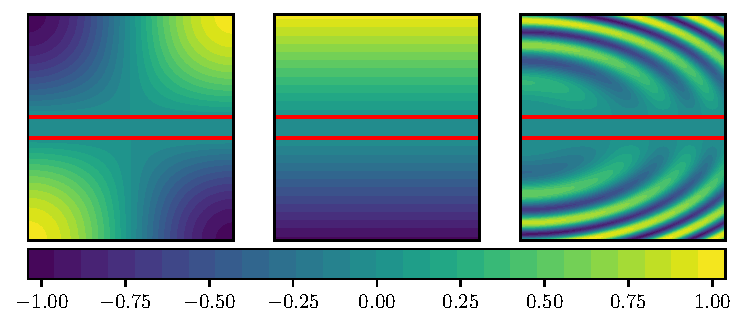
\includegraphics[scale=0.75]{Diagram_GradZeroIllustrations.pdf}
	\caption{\label{fig:Diagram_GradZeroIllustrations} Examples illustrating how non-zero gradients of zero can arise, with the region between the red lines representing an edge $I_{jk}$, which has been thickened so one can view the function values along this edge. Despite each of the functions appearing constant along the edge $I_{jk}$, and thus constant to the measure $\lambda_{jk}$, the function is changing in the direction $n_{jk}$ as it crosses $I_{jk}$ and it's behaviour ``off the edge" is unknowable from the perspective of $\lambda_{jk}$. }
\end{figure}
Indeed, the measure $\lambda_{jk}$ is unable to deduce whether (for $x\in I_{jk}$) $u(x+hn_{jk})$ is different from $u(x)$ for $h\neq0$, given the only information it can have about $u$ are its values on $I_{jk}$.
Consequentially, $\lambda_{jk}$ can have no concept of $\pdiff{u}{n_{jk}}$ --- changing the profile of $u$ across the edge $I_{jk}$ does not change $u$ on $I_{jk}$, and consequentially the component of any ``gradient" directed along $n_{jk}$ corresponds to no change in the function $u$ from the perspective of $\lambda_{jk}$, making this component a gradient of zero.
In contrast, the measure $\lambda_{jk}$ can evaluate expressions like $u(x+he_{jk})-u(x)$ --- that is, changes in the function along $I_{jk}$ are detected by the measure $\lambda_{jk}$.
Such changes correspond to $\pdiff{u}{e_{jk}}$ being non-zero, and thus we find that tangential gradients are directed along $e_{jk}$ (and provide a ``derivative" in this direction too).
This also highlights the reason for defining the gradients of zero and tangential gradients as in section \ref{sec:BorelMeasSobSpaces} --- given a tangential gradient $\ktgrad_{\lambda_{jk}}u$, $\lambda_{jk}$ can reconstruct the function $u$ along the edge $I_{jk}$, but cannot determine what $u$ is doing across $I_{jk}$.
Ergo, every function has a gradient that is unique up to a gradient of zero, because there is no way for $\lambda_{jk}$ to determine what $u$ looks like across (and thus outside of) $I_{jk}$.

The above story is similar when considering the tangential gradient of $u$ with respect to the measure $\nu$.
Here, the ``view" of the measure is even more restricted, only being able to view the value of $u$ at the vertices, which are a set of isolated points in $\ddom$.
As such, there is no way for the measure $\nu$ to reconstruct any kind of sensible gradient --- there are no ``nearby" function values $u\bracs{v_j + h x}, x\neq 0$ to compare the value of $u\bracs{v_j}$ to.
The result is corollary \ref{cory:NuTangGradChar}, any gradient must be a gradient of zero, because as far as $\nu$ is concerned, there is no visible change in $u$ in any neighbourhood of $v_j$.
Then, given that $\dddmes$  is just the sum of the measures $\ddmes$ and $\nu$, we find that $\ktgrad_{\dddmes}u$ inherits the behaviours from $\ddmes$ and $\nu$.